% Created 2015-09-14 Mon 02:39
\documentclass{scrartcl}
\usepackage[utf8]{inputenc}
\usepackage[T1]{fontenc}
\usepackage{fixltx2e}
\usepackage{graphicx}
\usepackage{longtable}
\usepackage{float}
\usepackage{wrapfig}
\usepackage{soul}
\usepackage{textcomp}
\usepackage{marvosym}
\usepackage{wasysym}
\usepackage{latexsym}
\usepackage{amssymb}
\usepackage{hyperref}
\tolerance=1000
\usepackage[margin=18mm]{geometry}
\usepackage{amsmath}
\usepackage{graphicx}
\usepackage{subfigure}
\usepackage{parskip}
\usepackage{standalone}
\usepackage{tikz,pgf,pgfplots}
\usetikzlibrary{decorations.pathmorphing,patterns}
\usetikzlibrary{arrows,snakes,backgrounds,patterns,matrix,shapes,fit,calc,shadows,plotmarks,decorations.markings,datavisualization,datavisualization.formats.functions,intersections,external}
\pgfplotsset{compat=1.9}
\newcommand*{\mexp}[1]{\ensuremath{\mathrm{e}^{#1}}}
\newcommand*{\laplace}[1]{\ensuremath{\mathcal{L} \{#1\}}}
\newcommand*{\laplaceinv}[1]{\ensuremath{\mathcal{L}^{-1} \{#1\}}}
\newcommand*{\realpart}[1]{\ensuremath{\operatorname{Re}(#1)}}
\newcommand*{\impart}[1]{\ensuremath{\operatorname{Im}(#1)}}
\newcommand*{\vsp}[1]{\rule{0pt}{#1}}
\newcommand*{\tderiv}[1]{\ensuremath{\frac{d^{#1}}{dt^{n}}}}
\newcommand*{\bbm}{\begin{bmatrix}}
\newcommand*{\ebm}{\end{bmatrix}}
\newcommand*{\obsmatrix}{\mathcal{O}}
\newcommand*{\contrmatrix}{\mathcal{C}}
\newcommand*{\cwh}{\ensuremath{\cos \omega h}}
\newcommand*{\swh}{\ensuremath{\sin \omega h}}
\newcommand*{\zethree}{\big(z - \mexp{-3h}\big)}
\providecommand{\alert}[1]{\textbf{#1}}

\title{Computerized control - preparation for partial exam 1}
\author{Kjartan Halvorsen}
\date{\today}
\hypersetup{
  pdfkeywords={},
  pdfsubject={},
  pdfcreator={Emacs Org-mode version 7.9.3f}}

\begin{document}

\maketitle



\section*{The Nyquist criterion}
\label{sec-1}

The figure below shows the Nyquist curve for the open-loop pulse-transfer function 
\[ H(z) = \frac{0.25K}{(z-1)(z-0.5)} \]
for the case when $K=1$. 
\begin{center}
\includestandalone[width=0.4\linewidth]{nyquist}
\end{center}

(a) Indicate the phase marginal and the amplitude marginal in the figure.

(b) If the loop is closed as in the figure below, then for which values of $K$ is the closed-loop system stable?
\begin{center}
\includestandalone[width=0.4\linewidth]{feedback}
\end{center}
\section*{The Nyquist criterion and choice of sampling interval}
\label{sec-2}

The figure below shows the Nyquist curve for the continous-time system (dashed line)
\[ G(s) = \frac{1}{s(s+1)} \]
and for the corresponding discrete-time system sampled with different sampling periods: $h \in \{0.1, 0.4, 1 \}$. 
\begin{center}
\includestandalone[width=0.3\linewidth]{nyquist2}
\end{center}

(a) Describe briefly in own words how the Nyquist curve changes with increasing sampling period, and what this means for stability of the closed-loop system. 

(b) State the rule-of-thumb for choosing sampling period based on the Nyquist diagram.
\section*{Å\&W problem 2.10}
\label{sec-3}

The figure below shows a system of two tanks, where the input is the flow to the first tank and the output is the level in the second tank.
\begin{center}
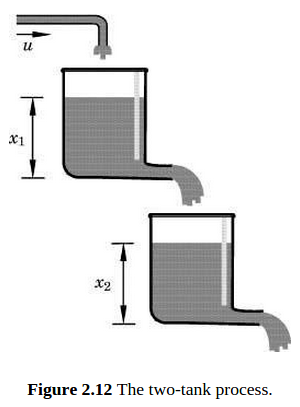
\includegraphics[width=0.2\linewidth]{tanks.png}
\end{center}
Use of the levels as state variables gives the system
\begin{align*}
\frac{dx}{dt} &= \bbm -0.0197 & 0\\0.0178 & -0.0129 \ebm x + \bbm 0.0263\\0 \ebm u\\
y &= \bbm 0 & 1\ebm x.
\end{align*}

(a) Sample the system with sampling period $h=12$.

(b) Verify that the pulse-transfer operator for the system is
\[ H(q) = \frac{0.030q + 0.026}{q^2 -1.65q + 0.68}. \]
\section*{Å\&W problem 3.2}
\label{sec-4}

Consider the closed-loop system below with
\[ H(z) = \frac{K}{z(z-0.2)(z-0.4)}. \]
\begin{center}
\includestandalone[width=0.4\linewidth]{feedback}
\end{center}

Determine the valuse of $K$ for which the closed-loop system is stable.
\section*{Å\&W problem 3.20}
\label{sec-5}


Given the system
\[ (q^2 + 0.4q)y(k) = u(k) \]

(a) For which values $K$ in the proportional controller 
\[ u(k) = K\big(u_c(k) - y(k)\big) \]
is the closed-loop system stable?

(b) Determine the stationary error $e = u_c-y$ when $u_c(k)$ is a step and $K=0.5$ in the controller in (a).
\section*{Solutions}
\label{sec-6}
\subsection*{The Nyquist criterion}
\label{sec-6-1}

   (a) The amplitude marginal is denoted $A_m$ and the phase marginal $\varphi_m$ in the figure below.
   \begin{center}
   \includestandalone[width=0.4\linewidth]{nyquist-solution}
   \end{center}
   
   (b) Since the open loop system $H(z)$ has no poles outside the unit disc (the pole in $1$ is excluded in the domain studied), the closed loop system \[H_c(z) = \frac{H(z)}{1+H(z)} \] will be stable as long as the nyquist curve does not encircle the point $-1$ on the negative real axis. The plot shows the nyquist curve for the system \[H_1(z) = \frac{1}{(z-1)(z-0.5)}.\] Since multiplication by a positive real value $K$ will only change the magnitude of each point on the curve, not the phase, the point of interest is the intersction with the negative real axis, and the corresponding amplitude marginal $A_m$. Wee see that the closed loop system will be stable as long as 
   \[\frac{K}{A_m} < 1, \] hence,
   \[K < A_m = 2, \]
   where the numerical value is obtained by visual inspection of the graph. The result also exemplifies the point of the amplitude marginal: It is the maximum amplification of the open loop system that is possible before the closed loop system becomes unstable.   
\subsection*{Nyquist criterion and sampling}
\label{sec-6-2}

   (a) The important changes in the nyquist curve when sampling the system are 
\begin{enumerate}
\item The curve intersects the real axis, so instability will occur for proportional control with high gain.
\item The phase marginal decreases with increasing sampling period $h$.
\end{enumerate}

   (b) The sampling period should be chosen so that the phase marginal is decreased by 5-15 degrees. 
\subsection*{For the problems from Å\&W, see the solution manual}
\label{sec-6-3}


   

\end{document}
